
\subsection{\sinterface}
The \astaff[] interface is illustrated in figure \ref{fig:staff_interface}.
After login, the \astaff[] is presented with the \textit{main} window. All the window have a back function which enables the \astaff[] to return to the previous window.


\subsubsection{Main}
The staff main window give the \astaff member access to all the functionality from the \astaff actor and from the \aclient actor. The \astaff have one button:
\begin{itemize}
	\item ``Worklist'' which directs the \astaff member to the ``Worklist'' window. 
\end{itemize}   
plus the menu button from the \aclient s main menu.

 After login the staff is presented with the ``Main'' staff window where the button ``Worklist'' is shown. When the ``Worklist'' button is press the window ``Worklist'' opens. 


\subsubsection{Worklist}
``Worklist'' contains a list with all the problems assigned to the staff member who is signed in. The list show the following properties: Name, Deadline, Priority, and ETA.


\subsubsection{Staff problem view}
The window ``Staff problem view'' shows information about a selected problem. The window contains a info field, a checkbox where the \astaff member can choose to subscribe to the problem, a text field with all the existing comments related to the problem, a text field where new comments can be entered, the button ``Add comment'' to send the entered comment, a text field containing entered solutions, the ``Reassign problem'' button which opens the ``Reassign problem to staff'' window, a checkbox to mark the problem as solved, a calender to set deadlines, the button ``Approve deadline'' to approve a suggested deadline if one is suggested and changes and the button ``Delete'' to remove the problem from the system.   

\subsubsection{Solution view}
The solution view 

\subsubsection{Staff problem view}




\subsubsection{Add solution}

%\subsubsection{Select assignees}


\begin{comment}
The solve problem interface is used by the \astaff[] to perform his daily duties. This is the interface he will be using to get his \todolist{}, to communicate with the \aclient{} and to solve the problems.
Since the \astaff{} often acts as \sadmin{} the button to go to the administration interface is presented at the main window of the \spinterface{}.
But only the \astaff{} with the correct permissions can enter.
The main window contains the \client{} main window, so \astaff{} has the same opportunities as \aclient{} plus the additional options, which har described below.


\subsubsection{Worklist Window}
The worklist window shows a list of unsolved problems assigned to the \astaff. From here he can select a problem to work with. 

\subsubsection{Problem View}
The problem view window contains all needed information about the selected problem. It contains the following buttons: 
\begin{itemize}
\item \textbf{Add comment}  takes the \astaff{} to the add comment window, where he can enter a comment and add to the selected problem. 

\item \textbf{Add solution} presents the \astaff{} for a searchable of problems. Every problem is a link that opens a simplified view of the problem with a button to attach solution. This button takes the \astaff{} back to problem view. From add solution the \astaff{} can press the button add new solution which takes him to a window where he can enter a solution description.
And add the new solution 

\item \textbf{Change assignment} button takes the \astaff{} to a window where he is presented with a list of all \staff{} in his departments. Every \staff{} has a checkbox attached. The selected elements presents the \staff{} assigned to the specific problem. Changing this and saving allows the \astaff{} to assign or reassign the \astaff{}. 

\item \textbf{Delete solution} If any solution is already attached each attached solution has a delete button to remove it from the problem. 

\item \textbf{Delete} button deletes the problem and returns the \staff{} to his worklist.

\end{itemize}
From any point in the interface the \astaff{} is able to logout or close the browser. 

\end{comment}

\begin{figure}[H]
	\centering
		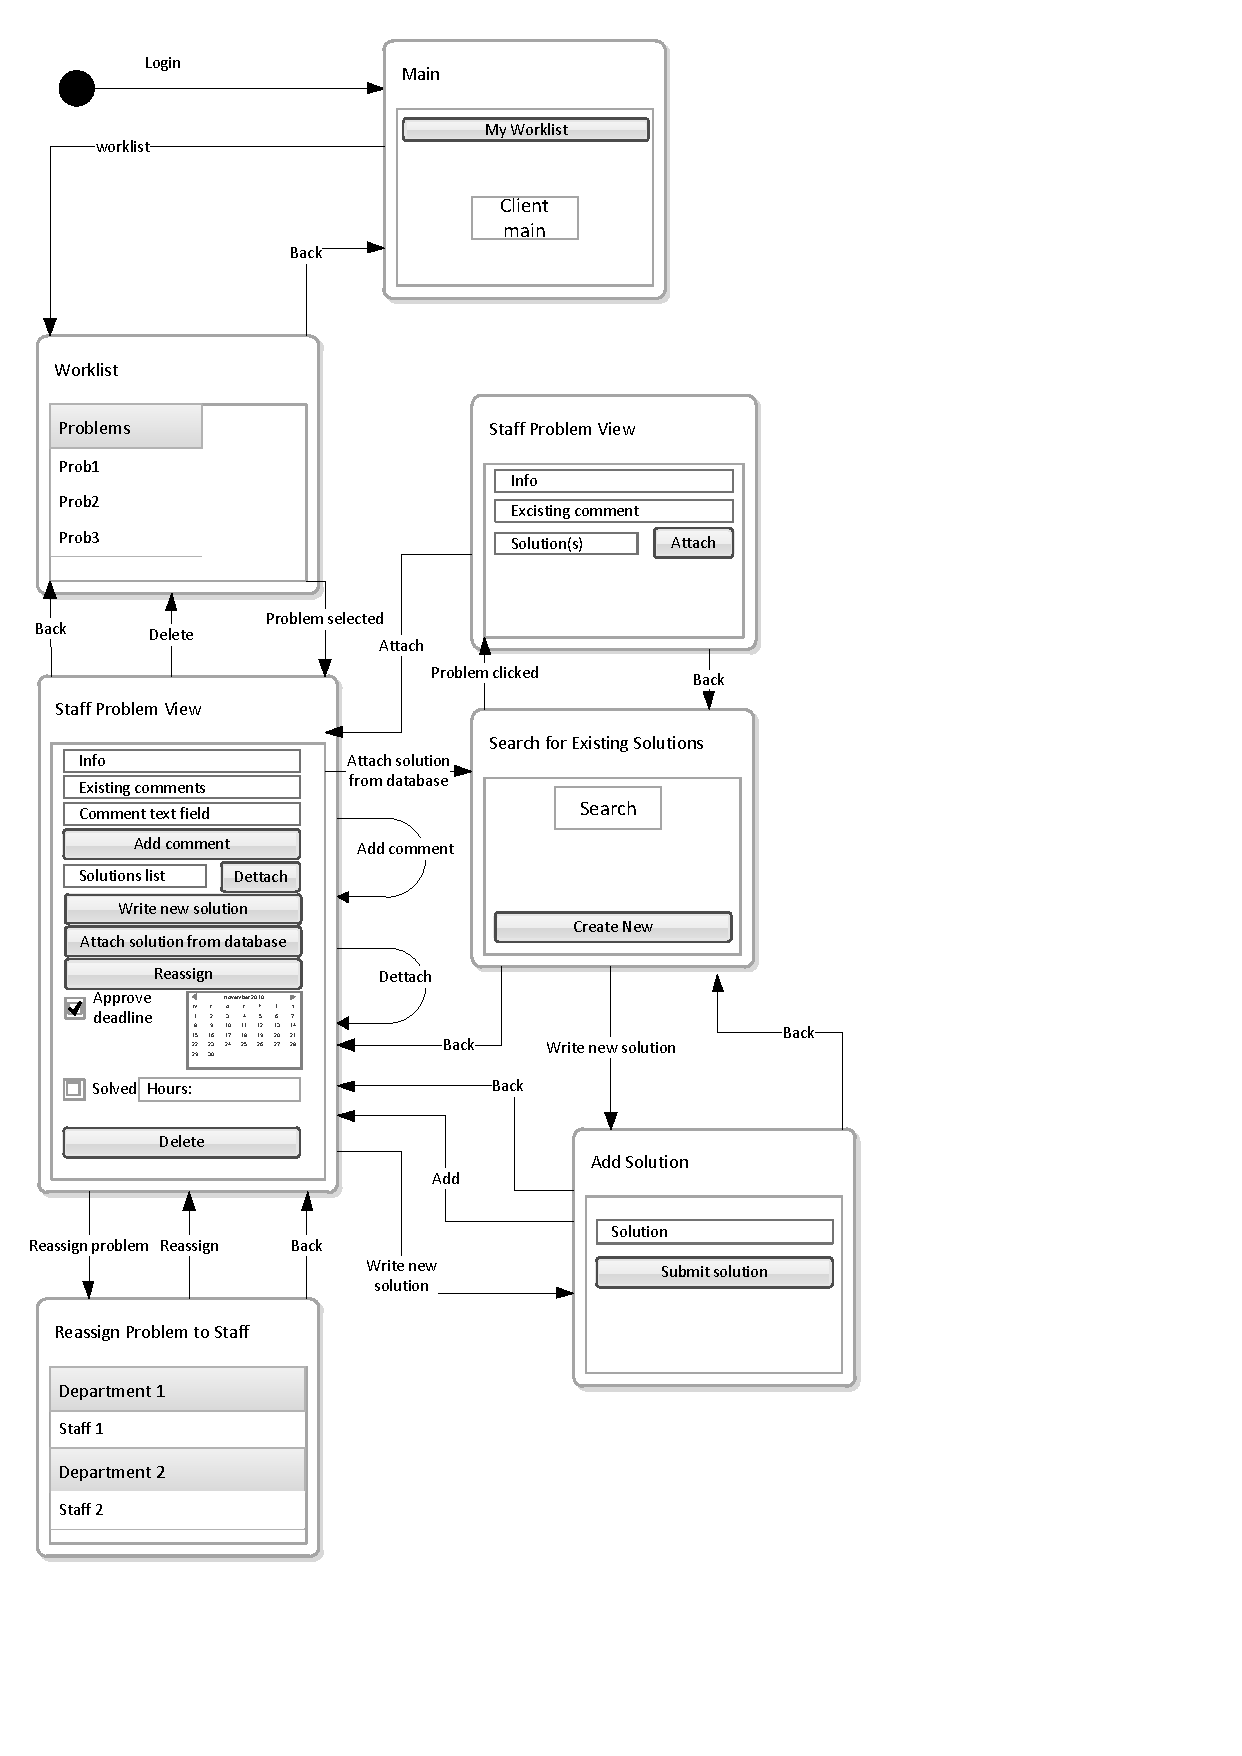
\includegraphics[width = \textwidth, clip=true, trim=0 4cm 5cm 0]{input/application_domain_analysis/Navigation_DiagramStaff.pdf}
	\morscaption{\sinterface[c]}
	\label{fig:Navigation_DiagramAdmin}
\end{figure}



